\documentclass[a4paper,11pt]{article}
\usepackage[total={148mm,230mm}]{geometry}
\usepackage[T1]{fontenc}
\usepackage[utf8]{inputenc}
%\usepackage{lmodern}
\usepackage{amsmath}
\usepackage{hyperref}
\usepackage{tikz}
\usepackage{listings}
\usepackage[english,ngerman]{babel}
\usepackage{graphicx}
\usepackage{xcolor}
\usepackage{caption}
\usepackage{apacite}

\definecolor{codegreen}{rgb}{0,0.6,0}
\definecolor{codegray}{rgb}{0.5,0.5,0.5}
\definecolor{codepurple}{rgb}{0.58,0,0.82}
\definecolor{backcolour}{rgb}{0.95,0.95,0.92}

\lstdefinestyle{cplusplus}{
    backgroundcolor=\color{backcolour},   
    commentstyle=\color{codegreen},
    keywordstyle=\color{magenta},
    numberstyle=\tiny\color{codegray},
    stringstyle=\color{codepurple},
    basicstyle=\ttfamily\footnotesize,
    breakatwhitespace=false,         
    breaklines=true,                 
    captionpos=b,                    
    keepspaces=true,                 
    numbers=left,                    
    numbersep=5pt,                  
    showspaces=false,                
    showstringspaces=false,
    showtabs=false,                  
    tabsize=2
}

\lstset{style=cplusplus}

\newcommand{\CC}{C\nolinebreak\hspace{-.05em}\raisebox{.4ex}{\tiny\bf +}\nolinebreak\hspace{-.10em}\raisebox{.4ex}{\tiny\bf +}\hspace{.1em}}

\title{Vergleich der Komplexität von \break Tree-Search-Algorithmen}
\author{}


\begin{document}

\maketitle
\thispagestyle{empty}
\pagebreak
\selectlanguage{english}
\begin{abstract}
In diesem Projekt wird die Komplexität von verschiedenen einfachen Tree-Search-Algorithmen untersucht. Es werden verschiedene Algorithmen wie die Tiefensuche, Breitensuche und andere heuristische Suchalgorithmen auf binären Suchbäumen getestet. Dabei wird die Anzahl der durchsuchten Knoten und die benötigte Zeit gemessen, um die Effizienz der Algorithmen zu vergleichen. Das Ziel ist es, die Komplexität der Suchalgorithmen zu berechnen, um diese dadurch zu vergleichen.
\end{abstract}
\selectlanguage{ngerman}
\pagebreak
{%https://tex.stackexchange.com/a/306617
  \hypersetup{hidelinks}
  \tableofcontents
}
\pagebreak

%TODO: aus der Sicht einer 3. Person / Passiv schreiben!!
%TODO: alle begriffe, die oft vorkommen, gleich schreiben: z.B. Tree-Search Algorithmus (angang immer gross, verbunden)
%TODO: es ist kein suchbaum, den wir benutzt haben, sondern ein normaler baum -> ändern

\section{Einleitung}
Das Ziel dieses Projekts ist es, die Komplexitäten verschiedener Tree-Search-Algorithmen hinsichtlich der Größe und Tiefe des Baumes zu vergleichen. Dabei wird ein Programm in der Programmiersprache \CC erstellt, um die Berechnungen zu messen und zu überprüfen. 

Tree-Search-Algorithmen sind in der künstlichen Intelligenz weit verbreitet und werden verwendet, um Entscheidungsprobleme zu lösen. Da verschiedene Algorithmen unterschiedliche Vorteile und Nachteile aufweisen, ist es wichtig, ihre Leistungsfähigkeit und Komplexität zu verstehen. Eine Art, dies zu messen ist die Einschätzung der Komplexität. Diese ist eine Abschätzung für das obere Limit der Laufzeit eines Tree-Search-Algorithmus bei einer Anzahl von $n$ und einer Tiefe von $d$ Knoten. In diesem Projekt wird die Komplexität von verschiedenen Tree-Search-Algorithmen miteinander verglichen, um eine bessere Einschätzung der Komplexität bei der Verwendung dieser Algorithmen zu ermöglichen.


\section{Theorie}
\subsection{Baum}
Suchbäume sind Datenstrukturen aus der Graphentheorie. Der Begriff 'Suchbaum' bezieht sich darauf, dass die Datenstruktur baumartig organisiert ist. Ein Baum besteht aus einer Wurzel, die den obersten Knoten (engl. nodes) darstellt, und einer Anzahl von Zweigen oder Kanten, die von der Wurzel zu den Blättern führen, die die Endpunkte des Baums darstellen. Jeder Knoten im Baum repräsentiert eine Entscheidung oder einen Zustand, und jeder Zweig repräsentiert eine Aktion, die von diesem Zustand aus ausgeführt werden kann.

%TODO: package für anführungszeichen hinzufügen

Ein Baum ist also ein zusammenhängender Graph, der keine geschlossenen Pfade enthält \cite{graphs}, d.h. der sich nur in eine Richtung von der Wurzel aus erstreckt.

\subsubsection{binärer Baum}

EIn binärer Baum ist eine besondere Art von Baum, bei dem jeder Knoten maximal zwei Kindknoten (engl. \emph{child nodes}) haben kann. Ein solcher Baum ermöglicht eine effizientere Suche, da Suchalgorithmen sich an der Baumstruktur orientieren können, um die Suche zu optimieren und dadurch schneller Ergebnisse zu liefern. 

Ein binärer Baum kann ausgeglichen/balanciert, teilweise balanciert oder unbalanciert sein. Wenn er ausgeglichen ist, bedeutet dies, dass beide Teilbäume eines Knotens (links und rechts) immer gleich Tief sind, während bei unbalancierten Bäumen die Tiefe der Teilbäme sich beliebig unterschieden kann. Bei einem unbalancierten binären Baum kann zum Beispiel ein Teilbaum vollständig leer sein, während beim anderen alle Knoten sind. Ein teilweise balancierter Baum üerschreitet eine gewisse Tiefendifferenz der Teilbäme nicht.
%TODO "/" zeichen entfernen, Zitieren?

\subsubsection{binärer Suchbaum}
Bei einem binärer Suchbaum kann jeder Knoten nur zwei Kindknoten haben. Ausserdem erfordert ein binärer Suchbaum, im Gegensatz zu einem normalen Suchbaum, eine bestimmte Anordnung der Knoten: Diese sind so angeordnet, dass jeder Knoten kleiner als alle Knoten im rechten Teilbaum ist, aber grösser als alle Knoten im linken Teilbaum ist \cite{c2_algorithms}.
%TODO: letzten Satz besser formulieren / restliche Theorie ist im Plural geschrieben, hier auch ändern? -> nach oder vor Punkt Zitieren?

Der Vorteil dieser speziellen Anordnung ist, dass man schnell einen Knoten im Baum finden kann, da mit jedem durchlaufenen Knoten der Suchraum, also der Bereich, in dem nach einem bestimmten Knoten gesucht wird, durch das Vergleichen von Schlüsselwerten immer weiter eingeschränkt und halbiert werden kann. Auch ist das Einfügen und Löschen von Knoten aus dem Baum einfacher. 

\subsection{Tree-Search Algorithmus}
Tree-Search-Algorithmen sind eine Art von Algorithmen, die zur Lösung von Suchproblemen verwendet werden. Sie sind nützlich, wenn aus einer grossen Anzahl von möglichen Optionen die passende gefunden werden muss.
%TODO: passenden?

Tree-Search-Algorithmen arbeiten mit Suchbäumen, in denen die verschiedenen Optionen als Knoten, die über Kanten verbunden dargestellt sind. Die Suche nach der Lösung des Problems besteht darin, durch die Baumstruktur zu navigieren und den Pfad zu finden, der von der Wurzel (engl. root) bis zum Zielzustand führt.
%TODO: Zustand oder Option?

\subsection{Komplexität von Tree-Search-Algorithmen}
Das Durchsuchen eines Baumes nach einem gewünschten Zustand dauert nicht immer gleich lange. Es hängt vielmehr von einer Vielzahl verschiedener Faktoren ab, wie zum Beispiel der Größe und Tiefe des Suchbaumes oder der Anzahl der Knoten. Eine Abschätzung für die obere Schranke der Suchdauer und damit der Effizienz eines Tree-Search-Algorithmus gibt die Komplexität. 
%TODO: verzweigungsfaktor auch nennen?

Die Komplexität von Tree-Search-Algorithmen wird in der sogenannten $O$-Notation ausgedrückt, die angibt, wie schnell die Laufzeit eines Suchalgorithmus mit der Grösse eines Baumes wächst. Eine Komplexität von $O(n)$ bedeutet beispielsweise, dass die Laufzeit eines Algorithmus linear von der Anzahl der Knoten $n$ abhängt.

\section{Algorithmen im Vergleich}
Untersucht wurden verschiedene Tree-Search-Algorithmen, unter anderem die Tiefensuche (engl. depth-first search, DFS), die Breitensuche (engl. breadth-first search, BFS) und die Monte-Carlo-Baumsuche (engl. Monte Carlo tree search, MCTS). Die Komplexität wurde zunächst für jeden Suchalgorithmus berechnet und anschliessend mit dem Programm in Bezug auf die Anzahl der Baumknoten und die Tiefe, in der das Ergebins lag, überprüft.
%TODO: untersucht -> umformulieren, mathematisch berechnet -> umformulieren

\subsection{Der Suchbaum}
Das Projekt wurde mit einem binären Suchbaum umgesetzt, da diese Baumart den Vorteil hat, leicht skalierbar zu sein. Auch ist die Tiefe des Baumes logarithmisch zu der Anzahl der Knoten, was die Regelung der Baumtiefe erleichtert. Da jeder Knoten zwei \emph{child}-Knoten enthält, ist die Tiefe $d$ eines binären Baumes mit $n$ Knoten $$d \approx \log_2(n)$$ \cite{c2_algorithms}. %\text{.}
%TODO: ist die automatische Tiefe ein Vorteil?
%TODO: stimmt das Zitat?

Der Baum wurde wie folgt umgesetzt: Der Baum besteht aus einzelnen Knoten, die aus einem \emph{struct}-Datentyp bestehen, der über Pointer auf die \emph{child}- und \emph{parent}-Knoten verweist.

\lstinputlisting[language=C++, firstline=16, lastline=23]{../src/BinaryTree.h}

Der Vorteil einer solchen Struktur ist, dass einzelne Knoten leicht geändert werden können. Zusätzlich beschleunigt eine solche Implementierung den Aufruf der einzelnen Knoten, was die Gesamtlaufzeit des Programms verkürzt. Messungen haben ergeben, dass bei dieser Umsetzung die Knoten etwa mit $$O(Knoten) \approx O(1)$$ aufgerufen werden können, daher wurde diese Komplexität für die folgenden Rechnungen benutzt.


\subsection{Breitensuche}

Die Breitensuche (engl. Breadth-First-Search, BFS) ist ein ein Tree-Search Algorithmus, der Graphen schichtweise durchsucht, beginnend bei einem Startknoten und sich schrittweise auf benachbarte Knoten ausbreitet (Abbildung \ref{fig:binary_tree_bfs}).
%TODO: soll das in der Theorie stehen?

\begin{figure}[htbp]
\centering
\begin{tikzpicture}[level distance=1.5cm,  level 1/.style={sibling distance=3cm},  level 2/.style={sibling distance=1.5cm},  every node/.style={circle, draw}]
  \node (A) {A}
    child {node (B) {B}
      child {node (D) {D}}
      child {node (E) {E}}
    }
    child {node (C) {C}
      child {node (F) {F}}
      child {node (G) {G}
        child {node (H) {H}}
      }
    };
  
  \draw[red,very thick] (A)--(B)--(C)--(D)--(E)--(F)--(G)--(H);
\end{tikzpicture}
\caption{Der Breitensuchalgorithmus auf einem binären Baum, rot dargestellt}
\label{fig:binary_tree_bfs}
\end{figure}

Der im Programm gebrauchte Algorithmus benutzte eine \emph{Queue}, also eine Warteschlangen-Datenstruktur für die Speicherung des Baumes. Dabei werden jeweils alle Knoten in einer Schicht nacheinander durchsucht, auf \emph{child}-Knoten untersucht und anschliessend in die \emph{Queue} gespeichert. Dies wiederholt sich bis zum Baumende.

Die schichtweise Suche sorgt dafür, dass Knoten in gleicher Entfernung vom Startknoten zuerst besucht werden, bevor Knoten in weiter entfernten Schichten besucht werden. Dies ist besonders effizient bei flachen Bäumen.
%TODO: rechnung für Geschw.

\subsubsection{Berechnung der Komplexität}

Die Komplexität der Breitensuche in einem binären Baum mit Tiefe $d$ und $n$ Knoten beträgt:

\begin{align}
\text{Komplexität} &= \sum_{i=0}^{d} \text{Laufzeit der Ebene } i \\
&= \sum_{i=0}^{d} O(\text{Anzahl der Knoten in Ebene }i) \\
&= O(\sum_{i=0}^{d} \text{Anzahl der Knoten in Ebene }i) \\
&= O(\sum_{i=0}^{d} 2^1) \\
&= O(2^d) \\
&= O(n),
\end{align}

da die Breitensuche jeden Knoten höchstens einmal speichert. Der Speicherplatzbedarf für die \emph{Queue} beträgt also im schlechtesten Fall, wenn der gesuchte Wert in den tiefsten Blättern ist und alle anderen Knoten zuvor durchgegangen werden müssen $$O(n)$$, da die \emph{Queue} alle Knoten speichern muss, die besucht werden.Daher ist die Laufzeit der Breitensuche proportional zur Grösse des Baumes, also zur Anzahl Knoten.

Die Tiefe des Baumes hat auch einen Einfluss auf die Laufzeit, da die Suche mehr Knoten besuchen muss, bevor die Blätter erreicht werden. Da in dieser Umsetzung die Aufrufzeit der Knoten unabhängig von der Tiefe $O(1)$ ist, bleibt die Laufzeit aber immer noch proportional zur Anzahl der Knoten.

Dies wurde jedoch für einen unbalancierten Baum berechnet. Diese Komplexität gilt auch für ausbalancierte Bäume, doch da die Suche einen Knoten abbricht, sobald er gefunden wurde, ist die durchschnittliche Komplexität in einem ausbalancierten Baum kleiner, da weniger leere Knoten durchlaufen werden müssen. Dann der Durchschnitt $$O(\log_2(n)).$$
%TODO: begründen

\subsection{Tiefensuche}

Die Tiefensuche (engl. Depth-First-Search, DFS) ist ein Tree-Search Algorithmus der einen Graphen in die Tiefe durchsucht, d.h. sie geht so weit wie möglich in einen Pfad, bevor sie sich umwendet und nach anderen Pfaden sucht (Abbildung \ref{fig:binary_tree_dfs}).

\begin{figure}[htbp]
\centering
\begin{tikzpicture}[level distance=1.5cm,  level 1/.style={sibling distance=3cm},  level 2/.style={sibling distance=1.5cm},  every node/.style={circle, draw}]
  \node (A) {A}
    child {node (B) {B}
      child {node (D) {D}}
      child {node (E) {E}}
    }
    child {node (C) {C}
      child {node (F) {F}}
      child {node (G) {G}
        child {node (H) {H}}
      }
    };
  
  \draw[red,very thick] (A)--(B)--(D)--(E)--(C)--(F)--(G)--(H);
  
\end{tikzpicture}
\caption{Der Tiefensuchalgorithmus auf einem binären Baum, rot dargestellt}
\label{fig:binary_tree_dfs}
\end{figure}

Der für das Projekt geschriebene Algorithmus verwendet eine \emph{stack}-Datenstruktur, um die Reihenfolge der besuchenden Knoten zu speichern. Dabei wird ein Pfad durch den Baum gewählt, der bis zum einem Blatt begangen wird. Danach wird der Algorithmus bis zum letzten nicht vollständig erforschten Knoten zurückgeführt, von wo die Suche nochmals beginnt. Dieser Vorgang wird fortgesetzt, bis alle Knoten besucht wurden.
%TODO: soll stack, queue erklärt werden?
%TODO: soll code gezeigt werden?

\subsubsection{Berechnung der Komplexität}

Die Tiefensuche läuft alle Pfade des Baumes nacheinander in die Tiefe durch. Wenn der Baum nicht ausbalanciert ist, kann es passieren, dass ein Pfad von der Wurzel zu einem Blatt eine Länge von $n$ hat. Dann muss die Suche im schlechtesten Fall alle Knoten durchlaufen und hat damit ebenfalls eine Komplexität von $$O(n).$$

Die Tiefe ändert auch bei der Tiefensuche die Komplexität nicht, da alle Knoten innerhalb von $O(n)$ aufgerufen werden können.

Wenn der Baum ausbalanciert ist, beträgt die durchschnittliche Komplexität wie bei der Breitensuche $$O(\log_2(n)),$$ da in allen Teilbäumen gleich viele Knoten sind.
%TODO: leicht kurz. besser begründen?

\subsection{Monte-Carlo Baumsuche}

Die Monte-Carlo Baumsuche ist ein Algorithmus welcher auf der Monte-Carlo Methode basiert. Die Monte-Carlo Methode ist ein Verfahren welches mit einer grossen anzahl von Zufallsexperimenten welche basiert auf gegebenen Warscheinlichkeiten einen gesuchten Wert annähert.
%Bild der Montecarlo methode
Der Suchalgorithmus nutzt dieses Prinzip um zu entscheiden, welchen Pfad der algorithmus absucht. Genauer gesagt gibt es für jeden pfad eine Warscheinlichkeit die bestimmt wie hoch dei Chance ist, dass jene Pfad gewählt wird. Da die Monte-carlo Baumsuche wie eine modifizierte Tifensuche ist, wird immer bis zum ende des Baumes oder bis zur vorgegebenen Tiefe gesucht. Wenn der Algorithmus auf seinem Weg nicht den Gesuchten Wert findet, startet er seine Suche bei der niedrigsten Tiefe bei der noch nicht alle Wege analysiert wurden. 

\subsubsection{Berechnung der Komplexität}

Die Komplexität des Algorithmus ist $O(nI)$ um alle Knoten zu durchlaufen. I ist dabei das Produckt aller Gegenwarscheinlichkeiten die eintreffen müssten um zu diesem Ort zu gelangen ist. Bei einem ausbalanciertem Baum ist dabei die Komplexität $O(nI/2)$ da wir keine gegebene Warscheinlichkeiten für den Baum haben und diese zufällig generiert werden. Wären jedoch die Warscheinlichkeiten, dass ein Gesuchter Wert an einem bestimmten Ort wäre, hätte der Baum eine Warscheinlichkeit von $O(nI)$ wobei hier I kleiner ist und somit auch die Zeitkomplexität sinkt. 
Um die Gesamtzeit zu berechnen, nutzt man die Formel $$ t(n,l,d) = I*n*(\sum_{k=0}^{n} s^k) + O(m)$$ O(m) ist dabei die Zeitkomplexität des Zufalsgenerators für den Algorithmus.

\section{Resultate}
Bei allen Suchalgorithmen wurde die Laufzeit in Abhängigkeit von der Tiefe des Baumes und der Grösse des Baumes gemessen. Bei der Tiefe wurde ein Baum mit $5'000'000$ Knoten benutzt, bei der Grösse Bäume zwischen $1'000$ und $5'000'000$ Knoten. Alle Messungen wurden $100$ Mal durchgeführt, um allfällige Fehler auszugleichen, angezeigt wird jeweils der Durchschnitt der Messungen. Eine grössere Anzahl an Knoten oder Messungen war wegen der begrenzten Rechenleistung der benutzten Geräte nicht möglich; selbst die folgenden Messungen haben jeweils mehr als 45 Minuten gebraucht.

\subsection{Breitensuche}
	\begin{figure}[ht]
		\centering
		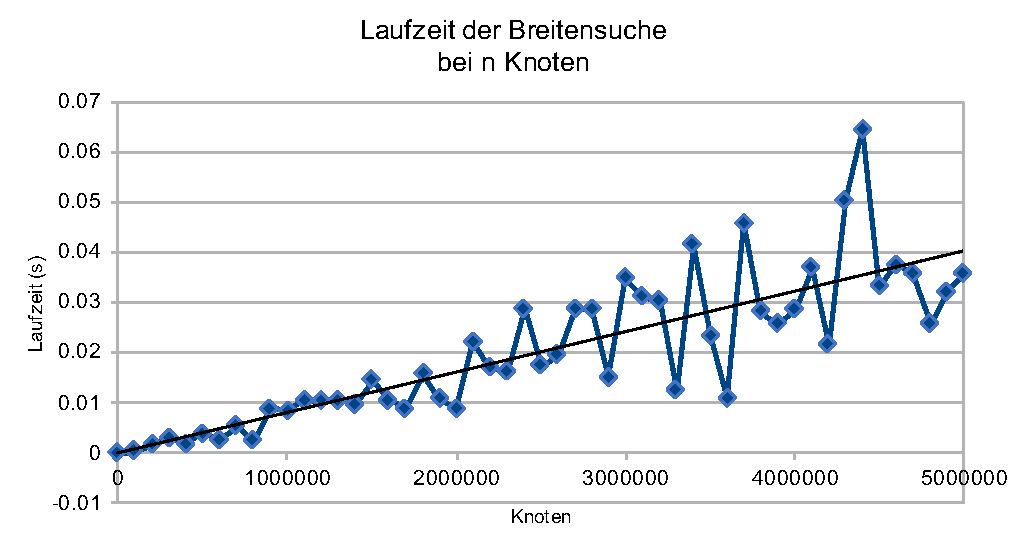
\includegraphics[width=0.85\linewidth]{img/BFS_size.pdf}
		\caption{Die Laufzeit der Breitensuche, abhängig von der Anzahl Knoten}
		\label{fig:bfs_time}
	\end{figure}
	
Die gemessenen Laufzeiten der Breitensuche stimmen ziemlich gut mit der Theorie überein (Abblidung \ref{fig:bfs_time}): Die Laufzeit steigt linear mit der Anzahl der Knoten, da die gemessenen Bäume jeweils teilweise balanciert sind. Die Ursache der Abweichungen ist die unterschiedliche Balancierung der Bäume.
\subsection{Tiefensuche}

	\begin{figure}[ht]
		\centering
		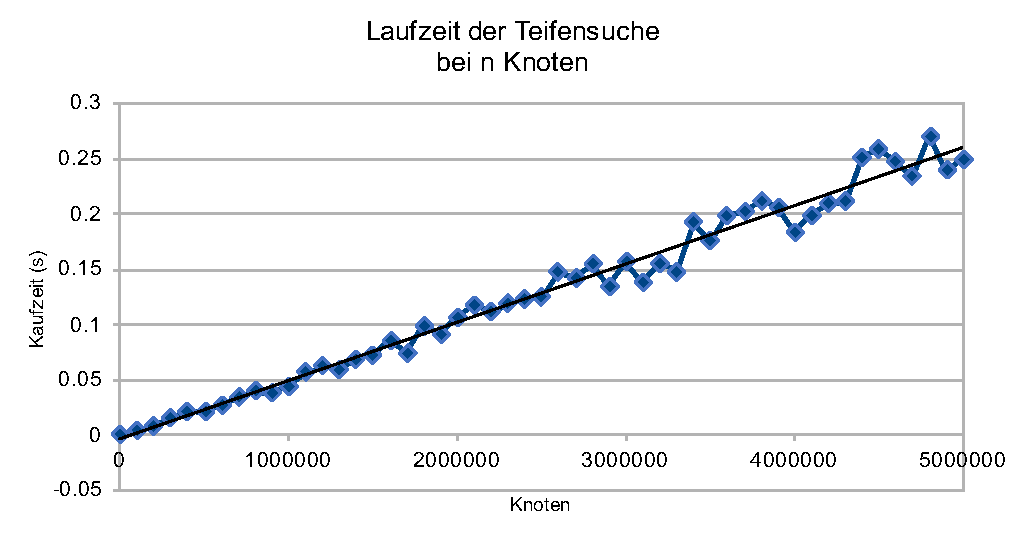
\includegraphics[width=0.85\linewidth]{img/DFS_size.pdf}
		\caption{Die Laufzeit der Treitensuche, abhängig von der Anzahl Knoten}
		\label{fig:dfs_time}
	\end{figure}
	%TODO: kaufzeit zu laufzeit umschreiben
	
Die gemessenen Laufzeiten der Tiefensuche stimmen sehr gut mit der Theorie überein, da die Laufzeit linear von der Kontenzahl $n$ abhängt (Abblidung \ref{fig:dfs_time}). Die grösseren Abweichungen die unterschiedliche Balancierungen der Bäume als Ursache: Aus Zeitgründen wurde für jede Knotenzahl nur ein Baum generiert, in dem $100$ Mal unterschiedliche Werte gesucht wurden. Falls ein Baum sehr unbalanciert ist, dauern alle $100$ Suchen durchschnittlich länger. Diese Unbalancierung ist bei grösseren Bäumen besser sichtbar als bei kleinen.

\subsection{Monte-Carlo Baumsuche}
s
	\begin{figure}[ht]
		\centering
		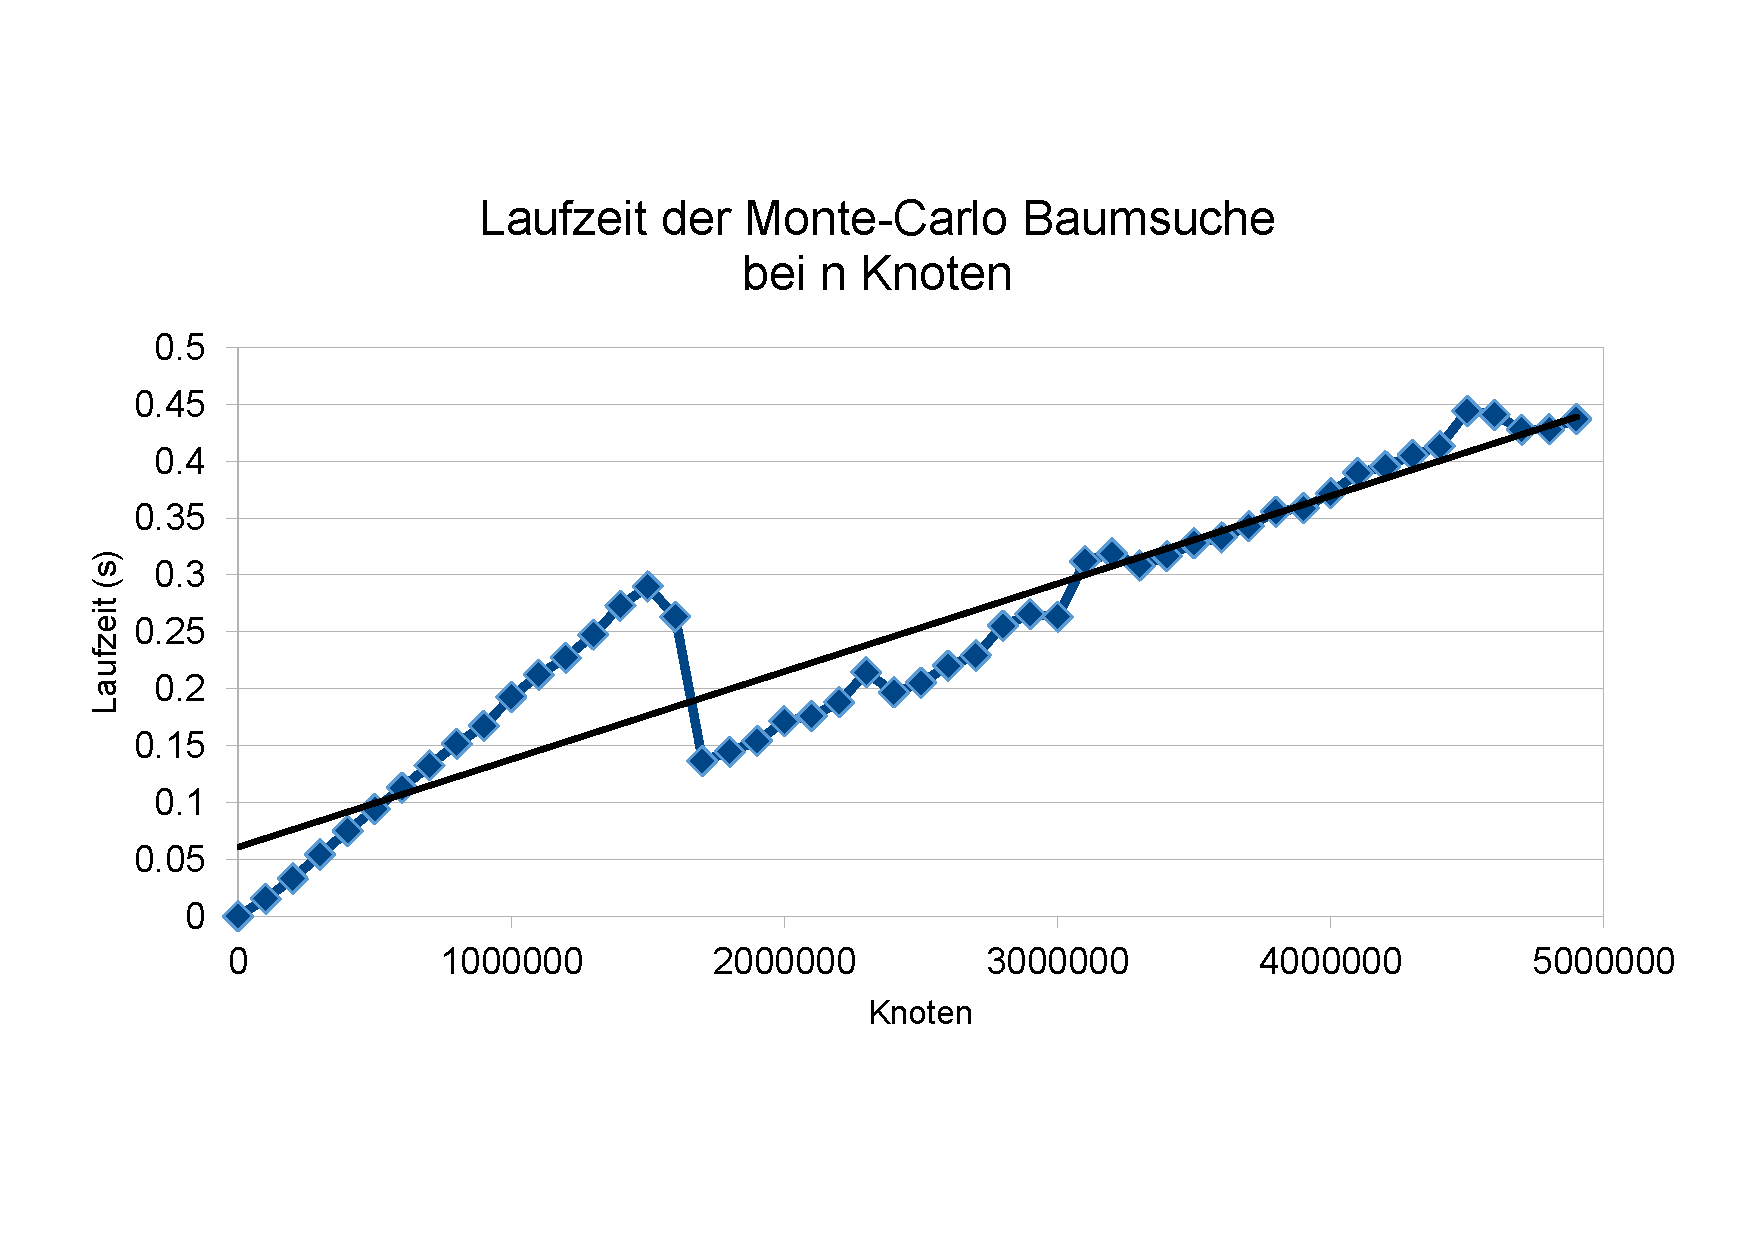
\includegraphics[width=0.85\linewidth]{img/MCTS_size.pdf}
		\caption{Die Laufzeit der Monte-Carlo Baumsuche, abhängig von der Anzahl Knoten}
		\label{fig:mcts_time}
	\end{figure}
\subsection{Vergleich}

\section{Schlussfolgerung}
\section{Reflexion}
Das Projekt, vor allem das Schreiben des Programms war ziemlich ansprochsvoll, ging aber gut. Eines der grössten Probleme war die Effizienz des Baumes. Der Code musste mehrmals umgeschrieben werden, um eine schnelle Aufrufezeit der einzelnen Knoten zu ermöglichen.

Als Schwierigkeit gestaltete sich auch das Generieren von Zufallszahlen, die man für die Knotenwerte und das Einfügen der Knoten in den Baum braucht. Zuerst verwendeten wir den Mersenne-Twister Pseudo-Zufallsgenerator, doch dieser war ausserordentlich langsam: um einen Baum mit 100'000 Knoten zu generieren brauchte es über 65 Sekunden. Durch den Einsatz des Xorshift128+ Pseudo-Zufallsgenerators konnte ein Baum gleicher Größe innerhalb von 20 Millisekunden generiert werden - das entspricht einer Geschwindigkeitssteigerung um mehr als das 3'000-fache! Allerdings war dieser Algorithmus nicht Teil der Standardbibliothek von \CC - er musste von uns implementiert werden.

Trotz diesen Optimierungen dauerten die Messungen für jeden der Suchalgorithmen mehr als 45 Minuten - insgesamt haben die Rechnungen mehr als 4 Stunden CPU-Zeit beansprucht. Trotzdem sind wir mit dem Projekt sehr zufrieden, da die Ergebnisse sehr gut den Theoriewerten entsprechen.

Der Quellcode für das Programm ist ist öffentlich, Open-Source und kann unter \href{https://github.com/Kepler-69c/binaryTree}{diesem Web-Link} aufgerufen werden.

\pagebreak
\bibliographystyle{apacite}
\bibliography{bibfile}


\end{document}
